
%----------------------------------------------------------------------------------------
%	PACKAGES AND THEMES
%----------------------------------------------------------------------------------------

\documentclass{beamer}
\usepackage[natbib=true,backend=biber, url=false, doi=false,isbn=false, maxbibnames=99, eprint=false, citestyle=authoryear-comp, maxcitenames=2]{biblatex}
\addbibresource{../../../bibliography.bib}
\usepackage{luatex85}
\usepackage{color, colortbl}
\definecolor{LRed}{rgb}{1,.8,.8}
\definecolor{MRed}{rgb}{1,.6,.6}
\definecolor{HRed}{rgb}{1,.2,.2}
\usepackage{tabularx}
\usepackage{tikz}
\usetikzlibrary{decorations}
\usetikzlibrary{patterns}
\usepackage{pgfplots}
\usepackage{appendixnumberbeamer}
\usepackage{caption}
\usepackage{subcaption}
\usepackage{booktabs}
%% If you'd like the default font size to be even larger, use 14pt or 17pt; these are supported by Beamer.
\usepackage{bbm}
\newcommand{\bbm}[1]{\mathbbm{#1}}
\newcommand{\bb}[1]{\mathbbm{#1}}
\usepackage[english]{babel}
\usepackage[utf8]{inputenc}
\usepackage[T1]{fontenc}
\usepackage{lmodern}
\usetikzlibrary{decorations.pathreplacing}
\setlength{\defaultaddspace}{2pt}
%%%%%%%%%%%%%%%%%%%%%%%%%%%%%%%%%%%%%%%%%
% These lines should usually go into a .sty file,
% but I'll leave them here so that it's easier to
% see how to customise a Beamer theme.
% Remember, the Beamer manual is your friend!!
% http://texdoc.net/pkg/beamer
%
%% So if your re-definitions have a @ somewhere, you
%% _MUST_ put a \makeatletter before these lines and then
%% \makeatother after them. This trick can only be done
%% in the preamble! BUT if you're doing these re-definitions
%% in a .sty file (so that you \usepackage it later), you
%% don't need the \makeatletter and \makeatother.
\makeatletter

%% Set the left and right margins
\setbeamersize{text margin left=1em,text margin right=1em}

%% FONTS
\setbeamerfont{title}{series=\bfseries,size=\LARGE}
\setbeamerfont{subtitle}{series=\bfseries,size=\Large}
\setbeamerfont{frametitle}{series=\bfseries,size=\small}
\setbeamerfont{block title}{series=\bfseries,size=\normalsize}
\setbeamerfont{footline}{size=\normalsize}

%% COLOURS
%% If you'd like everything to have the same colour
\usebeamercolor{black}
\setbeamercolor{normal text}{fg=black.fg}

%% Add a line after the frametitle
\addtobeamertemplate{frametitle}{}{\vspace*{-1ex}\rule{\textwidth}{1pt}}

%% Use circular discs as itemized list markers;
%% there's an existing option in Beamer for it so I'll use it
\setbeamertemplate{itemize items}[circle]

%% Remove default navigation symbols (We'll add the ones we need in the footline
\setbeamertemplate{navigation symbols}{}

\setbeamercolor{button}{bg=brown,fg=white}

%% And before the footline... actually we'd like to re-define
%% the footline
\setbeamertemplate{footline}{%
	%% Beamer headlines and footlines are always full-paperwidth, so if you want the horizontal line to
	%% not span it entirely you'll need to do a bit of arithmetic
	\centering
	\begin{minipage}{\dimexpr\paperwidth-\beamer@leftmargin-\beamer@rightmargin\relax}
		\centering
		\rule{\linewidth}{1pt}\vskip2pt
		\usebeamerfont{footline}%
		\usebeamercolor{footline}%
		%% The frame number smack in the middle
		\hfill\insertframenumber/\inserttotalframenumber
		\hfill%
		%% ONLY the navigation symbols we want at the far right.
		%% We use an \llap so that it takes up zero width, and doesn't throw the page number off-centre!
		\llap{\insertframenavigationsymbol\insertbackfindforwardnavigationsymbol}\par
	\end{minipage}\vskip2pt
}

\makeatother
%%%% END STYLE CUSTOMISATION %%%%%%%%%%%%

%\setbeamertemplate{footline} % To remove the footer line in all slides uncomment this line
%\setbeamertemplate{footline}[page number] % To replace the footer line in all slides with a simple slide count uncomment this line

%\setbeamertemplate{navigation symbols}{} % To remove the navigation symbols from the bottom of all slides uncomment this line


\newenvironment{wideenumerate}{\enumerate\addtolength{\itemsep}{16pt}}{\endenumerate}
\newenvironment{widelist}{\itemize\addtolength{\itemsep}{16pt}}{\enditemize}

\newcounter{saveenumi}
\newcommand{\seti}{\setcounter{saveenumi}{\value{enumi}}}
\newcommand{\conti}{\setcounter{enumi}{\value{saveenumi}}}
\AtBeginSection[]{
	\begin{frame}[noframenumbering]
	\vfill
	\centering
	\begin{beamercolorbox}[sep=8pt,center,shadow=true,rounded=true]{title}
		\usebeamerfont{title}\insertsectionhead\par%
	\end{beamercolorbox}
	\vfill
\end{frame}
}


\newcommand{\Tau}{\mathrm{T}}
\title{Part-time work while on unemployment insurance}
\author{Jeffrey Hicks \inst{1} }
\date[]{\today} 

\institute{\inst{1} UBC Economics 
}


\begin{document}
	{
		\setbeamertemplate{footline}{}	
		\begin{frame}[noframenumbering]
		\titlepage % Print the title page as the first slide
	\end{frame}
}

\begin{frame}{Why Care}


\begin{widelist}
	\item <1-> \textcolor{blue}{The Policy:} UI allows beneficiaries to keep a portion of part-time earnings.
	\item <2-> \textcolor{blue}{The Reason:} (1) Encourages self-insurance, and (2) "improves attachment to labour force".
	\item <3-> \textcolor{blue}{Unintended Consequence:} Discourages and crowds-out search for full-time work.
	\item <4-> \textcolor{blue}{Relevance:} "Gig" economy \textit{may} provide more opportunities for this form of part-time work.
\end{widelist}
\end{frame}


\begin{frame}
\begin{figure}
	\includegraphics[width=.9\linewidth]{../../figures/insurance_new_0.pdf}
\end{figure}
\end{frame}

\begin{frame}[noframenumbering]
\begin{figure}
\includegraphics[width=.9\linewidth]{../../figures/insurance_new_1.pdf}
\end{figure}
\end{frame}

\begin{frame}[noframenumbering]
\begin{figure}
\includegraphics[width=.9\linewidth]{../../figures/insurance_new2.pdf}
\end{figure}
\end{frame}

\begin{frame}[noframenumbering]
\begin{figure}
	\includegraphics[width=.9\linewidth]{../../figures/insurance_new3.pdf}
\end{figure}
\end{frame}

\begin{frame}{Research Questions}

\begin{widelist}
	
	\item<1-> \textcolor{blue}{\textbf{First-Stage:}} How does claw-back schedule affect \textcolor{blue}{part-time work}?

	\item <2-> \textcolor{blue}{\textbf{Second Stage:}} How does part-time work affect \textcolor{blue}{claim duration}?
	
	\item <3-> \textcolor{blue}{\textbf{Unfortunate Stage:}} How much do claimants \textcolor{blue}{mis-report} earnings?
	
	\item <4-> \textcolor{blue}{\textbf{Normative Question:}} Optimal design of part-time work incentives?
\end{widelist}
\end{frame}


\begin{frame}{Literature}
\begin{widelist}
	\item \textbf{Positive}: How program design affect behaviour. \textcolor{blue}{Schmieder 2016}.
	\item \textbf{Stepping-stone}: Part-time lead to full-time? \textcolor{blue}{Autor 2010}, \textcolor{blue}{Kyyra 2013}
	\item \textbf{Normative:} Optimal Benefit: \textcolor{blue}{Baily 1978} , \textcolor{blue}{Chetty 2006 }, \textcolor{blue}{Shimer 2007}, and \textcolor{blue}{Landais 2015}, Optimal Duration: \textcolor{blue}{Davidson 1997}, Optimal Training: \textcolor{blue}{Spinnewijn 2013}, Optimal Timing \textcolor{blue}{Kolsrud 2018 }, Optimal Take-Up \textcolor{blue}{Kroft 2008}, Optimal Cyclicality \textcolor{blue}{Kroft 2016, Saez 2018}
	\item \textbf{Partial insurance:} Extensive Margin: \textcolor{blue}{McCall 1996}, Intensive Margin: \textcolor{blue}{Barbanchon 2017}, Policy in Search Model: \textcolor{blue}{Ek 2015} 

\end{widelist}
\end{frame}

%\begin{frame}
%\begin{figure}\centering
%	\includegraphics[scale=.3]{../EI_data/WorkingWhileonClaim/figures/barbanchon.png}
%\end{figure}
%\end{frame}

\begin{frame}{Unemployment Insurance in Canada I}
\begin{widelist}
	\item Replacement rate = 55 percent.
	\item Voluntary quits and at-fault separations disqualified.
	\item Minimum hours threshold to qualify for benefits.
	\item Receive \textcolor{blue}{Entitlement Weeks} that can be used within a 52 week period.
	\item The qualifying threshold and entitlement weeks vary with regional unemployment rate.
\end{widelist}
\end{frame}


\begin{frame}{Two Types of Working While on Claim}
\begin{widelist}
	\item \textcolor{blue}{While Claiming:} Benefits and earnings simultaneously. Potential claw-back of benefit.
	\item \textcolor{blue}{While Postponing:} Take earnings, postpone benefit week.
\end{widelist}
\end{frame}

\begin{frame}{Two Types of Working While on Claim}
\includegraphics[width=.9\linewidth]{../../figures/weekly_participate_timetrends.pdf}
\end{frame}

\begin{frame}{Data}
\begin{wideenumerate}
	\item Universe of all Employment Insurance claims from 1996 to 2016 in Canada. \\
	\item Individuals \textcolor{blue}{linked across unemployment spells}.
	\item \textcolor{blue}{Weekly frequency}.
	\item Observe \textcolor{blue}{self-reported} earnings.
	\item Drawback: No post-claim outcomes visible.
	\item Take random sample of 1 million SIN numbers
\end{wideenumerate}
\end{frame}

\begin{frame}{Types of Claims}
\begin{table}\centering \caption{New Benefit Claims in 2014/2015}
	\begin{tabular}{lc}
		\toprule
		Regular &	1,342,610  \\ \addlinespace
		Fishing &	27,587\\ \addlinespace
		Work Sharing&	8024\\ \addlinespace
		Maternity&	169,080\\ \addlinespace
		Parental &	191,320\\ \addlinespace
		Sickness &	345,070\\ \addlinespace
		Compassionate Care &	6244\\ \addlinespace
		Parents of Critically Ill Children&	2846\\ \addlinespace
		\bottomrule
	\end{tabular}
\end{table}
\end{frame}


\begin{frame}{Earnings Allowance System}
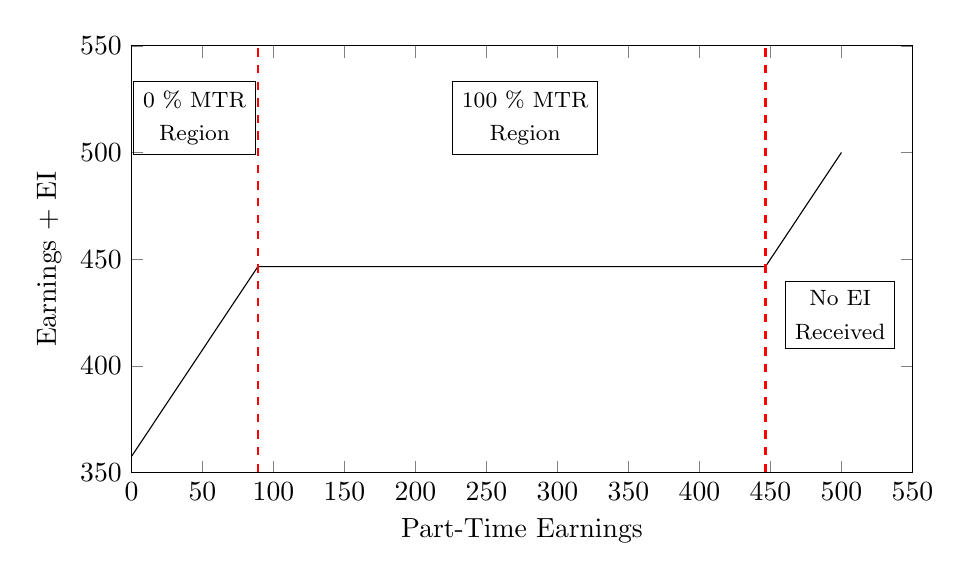
\begin{tikzpicture}
\begin{axis}[xlabel = Part-Time Earnings, ylabel = Earnings + EI, height = 7cm, width = 11.5cm, xmin=0, xmax = 550, ymin=350, ymax = 550]
\addplot[domain=0:550] coordinates { 
	(0,357.5)
	(89,446.5)
	(446.5, 446.5)
	(500,500)
};

\draw[red, thick, dashed] (89,0) -- (89,600);
\draw[red, thick, dashed] (446.5,0) -- (446.5,600);  
\end{axis}
\node[draw, align=center] at (.8, 4.5) {\footnotesize 0 \% MTR \\ \footnotesize Region};
\node[draw, align=center] at (5, 4.5) {\footnotesize100 \% MTR \\ \footnotesize Region};
\node[draw, align=center] at (9, 2) {\footnotesize No EI \\ \footnotesize Received};
\end{tikzpicture}
\end{frame}


\begin{frame}{Earnings Allowance System}
"Earnings Allowance":
\bigskip
\begin{widelist}
	\item \textcolor{blue}{Pre-2005:}  $T  = max\{ 25 \ \% \ of \ benefit, \ \$50 \}$ 
	\item \textcolor{blue}{2005-2008 Treatment:}  $T = max\{ 40 \ \% \ of \ benefit, \ \$75 \}$\
	\item \textcolor{blue}{Distance to Threshold:} Earnings minus Threshold (T)
\end{widelist}
\end{frame}


\begin{frame}
\begin{tikzpicture}
\begin{axis}[legend style = {at = {(.47,.9)}}, xlabel = Part-Time Earnings, ylabel = Earnings + EI, height = 8cm, width = 11.5cm, xmin=0, samples=50, xmax = 710]
\only<1->{
\addplot coordinates { 
	(0,357.5)
	(89,446.5)
	(446.5, 446.5)
	(700,700)
};
}
\only<2->{
\addplot coordinates { 
	(0,357.5)
	(143,500.5)
	(500.5, 500.5)
	(700,700)
};
}
\only<3->{
\addplot coordinates { 
	(0,357.5)
	(585,650)
	(650 ,650)
};
}
\legend{Original Schedule, 2005 to 2012 Schedule, Post-2012 Schedule}

\end{axis}{\tiny }
\end{tikzpicture}
\end{frame}


\begin{frame}{Maritime Regions}
\centering
	\includegraphics[width=.85\linewidth]{../../figures/maritimes_map.pdf}
\end{frame}

\begin{frame}{Ontario an Southern Quebec}
\centering
	\includegraphics[width=.85\linewidth]{../../figures/ontario_map.pdf}
\end{frame}

\begin{frame}{Prairies}
\centering
	\includegraphics[width=.85\linewidth]{../../figures/prairies_map.pdf}
\end{frame}

\begin{frame}{The most beautiful place on earth}
\centering
	\includegraphics[width=.85\linewidth]{../../figures/bc_map.pdf}
\end{frame}


\begin{frame}{Real or Reporting Responses?}
	\includegraphics[width=\linewidth]{../../figures/bunching_pres1.pdf}
\end{frame}

\begin{frame}{Real or Reporting Responses?}
\includegraphics[width=\linewidth]{../../figures/bunching_pres2.pdf}
\end{frame}

\begin{frame}{Dynamic Average Treatment Effects}
	Effect of Policy on Part-Time Work behavior \textcolor{blue}{(First-Stage)}:
	
		\begin{align}
		y_{i,q,r} &=  D_{i}\times \sum_{s} \textcolor{blue}{B_{s}}\times \bb{1}_{q=s} + \eta_q + \eta_r  +  \varepsilon_{i,q,r}
		\label{eq:dyn_weekly}
		\end{align}
	
\textcolor{blue}{Intuition:} Compare part-time work behavior on either side of treatment boundary.


\end{frame}

\begin{frame}{Average Earnings Threshold}
\includegraphics[width=\linewidth]{../../figures/earningsthresholds_timetrends_bytreatment.pdf}
\end{frame}


\begin{frame}{Participation Margin}
		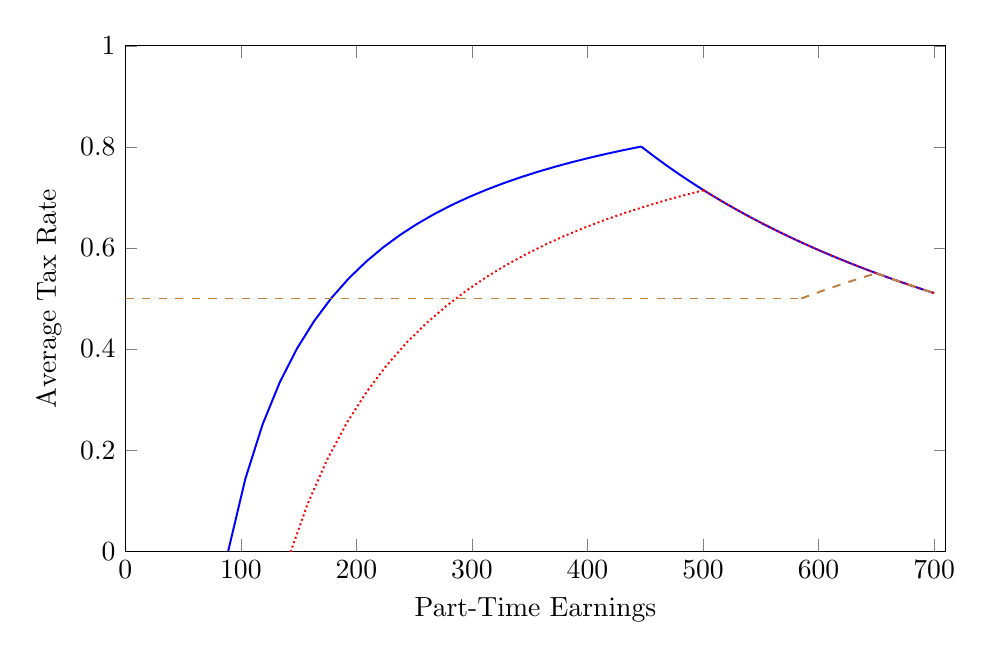
\begin{tikzpicture}
		\begin{axis}[xlabel = Part-Time Earnings, ylabel = Average Tax Rate, height = 8cm, width = 12cm, xmin=0, xmax = 710, ymin=0, ymax=1]
		\addplot[] coordinates {(0,0) (89,0)};
		\addplot [domain=89:446.5, blue, line width=0.25mm] {(x-89)/x};
		\addplot [domain=446.5:700, blue, line width=0.25mm] {(357.5)/x};
		\addplot[] coordinates {(0,0) (143,0)};
		\addplot [domain=89:500.5, red, densely dotted, line width=0.25mm] {(x-143)/x};
		\addplot [domain=500.5:700, red,densely dotted, line width=0.25mm] {(357.5)/x};
		\addplot [domain=0:585, brown, dashed,line width=0.25mm] {.5};
		\addplot [domain=585:650, brown, dashed, line width=0.25mm] {(585*.5 + x-585)/x};	
		\addplot [domain=650:700, brown,dashed, line width=0.25mm] {(357.5)/x};	
		\end{axis}
		\end{tikzpicture}
\end{frame}


\begin{frame}{Weekly Participation}
	\begin{figure} \centering
		\begin{subfigure}{.49\textwidth}\centering\caption{\footnotesize Prob of Working With Benefits}\label{map1}
			\includegraphics[width=\linewidth]{../../figures/dyn_did_weeklylevel_participate_withbenefit.pdf}	
		\end{subfigure}
		\begin{subfigure}{.49\textwidth}\centering\caption{\footnotesize Prob of Working Without Benefits}\label{map2}
			\includegraphics[width=\linewidth]{../../figures/dyn_did_weeklylevel_participate_nobenefit.pdf}	
		\end{subfigure}
	\end{figure}
$\beta = 1.5$, Base = 7 percent
\end{frame}

\begin{frame}{Weeks Worked Per Claim}
	\begin{figure}\centering
		\begin{subfigure}{.49\textwidth}\centering\caption{\footnotesize Worked Weeks With Benefits $>0$}\label{map1}
		\includegraphics[width=\linewidth]{../../figures/dyn_did_claimlevel_weeks_worked_withbenefit_i.pdf}	
	\end{subfigure}
	\begin{subfigure}{.49\textwidth}\centering\caption{\footnotesize Worked Weeks Without Benefits $>0$ }\label{map2}
		\includegraphics[width=\linewidth]{../../figures/dyn_did_claimlevel_weeks_worked_nobenefit_i.pdf}
	\end{subfigure}
	\end{figure}
$\beta = .9$, Base = 1.8
\end{frame}


\begin{frame}{Ever Worked During Claim}
\begin{figure}\centering
	\begin{subfigure}{.49\textwidth}\centering\caption{\footnotesize With Benefits}\label{map1}
	\includegraphics[width=\linewidth]{../../figures/dyn_did_claimlevel_ever_participate_withbenefit.pdf}	
	\end{subfigure}
	\begin{subfigure}{.49\textwidth}\centering\caption{\footnotesize Without Benefits}\label{map1}
		\includegraphics[width=\linewidth]{../../figures/dyn_did_claimlevel_ever_participate_nobenefit.pdf}	
	\end{subfigure}
\end{figure}
$\beta = 5.2$, Base = 33 percent
\end{frame}


\begin{frame}{Extensive Margin Summary}
\textcolor{blue}{Lesson:} Reported work participation increased on all extensive margins:

\bigskip
\bigskip

\textcolor{blue}{Caveat:} Simultaneous pilot --- best 14 weeks for benefit calculation, rather than 26 weeks $\rightarrow$ more incentive to take small work weeks.

\bigskip
\bigskip

\textcolor{blue}{Takeaway:} Large elasticity ---> implications for optimal claw-back system.
\end{frame}


\begin{frame}{Weekly Earnings Conditional on Working}
\begin{figure} \centering
	\begin{subfigure}{.49\textwidth}\centering\caption{\footnotesize Mean Earnings With Benefits}\label{map1}
	\includegraphics[width=\linewidth]{../../figures/dyn_did_weeklylevel_earn_amt_withbenefit.pdf}	
\end{subfigure}
\begin{subfigure}{.49\textwidth}\centering\caption{\footnotesize Mean Earnings Without Benefits }\label{map2}
	\includegraphics[width=\linewidth]{../../figures/dyn_did_weeklylevel_earn_amt_nobenefit.pdf}	
\end{subfigure}
\end{figure}
$\beta = 17.6$, Base = 155
\end{frame}

\begin{frame}{Total Earnings Throughout Claim}
\begin{figure} \centering
	\begin{subfigure}{.49\textwidth}\centering\caption{ \footnotesize Total Earnings With Benefits }\label{map2}
	\includegraphics[width=\linewidth]{../../figures/dyn_did_claimlevel_total_earn_withbenefit.pdf}	
	\end{subfigure}
	\begin{subfigure}{.49\textwidth}\centering\caption{ \footnotesize Total Earnings Without Benefits }\label{map2}
		\includegraphics[width=\linewidth]{../../figures/dyn_did_claimlevel_total_earn_nobenefit.pdf}	
	\end{subfigure}
\end{figure}
$\beta = 171.4$, Base =
\end{frame}

\begin{frame}{What is Driving the Average Effect?}
\begin{tikzpicture}
	\node {	\includegraphics[width=\linewidth]{../../figures/treatment2005_earningsw.pdf}};	
	\node[align=center] at (2, 2.4) {\shortstack{ \textcolor{blue}{Shifting of Bunching Mass:} \\  Reduced under-reporting or real behavior?}};
	\end{tikzpicture}
\end{frame}

\begin{frame}{Placebo}
		\includegraphics[width=\linewidth]{../../figures/placebo2005_earningsw.pdf}	
\end{frame}

\begin{frame}{Intensive Margin Summary}
\textcolor{blue}{Summary:} Positive intensive margin elasticity on all margins. 

\bigskip
\bigskip

\textcolor{blue}{Caveat:} Real or reporting response?

\bigskip
\bigskip

\textcolor{blue}{Next Step:} Credibly disentangle reporting from real.

\end{frame}

\begin{frame}{How to Separate the Magnitudes of Real and Reporting Responses?}
		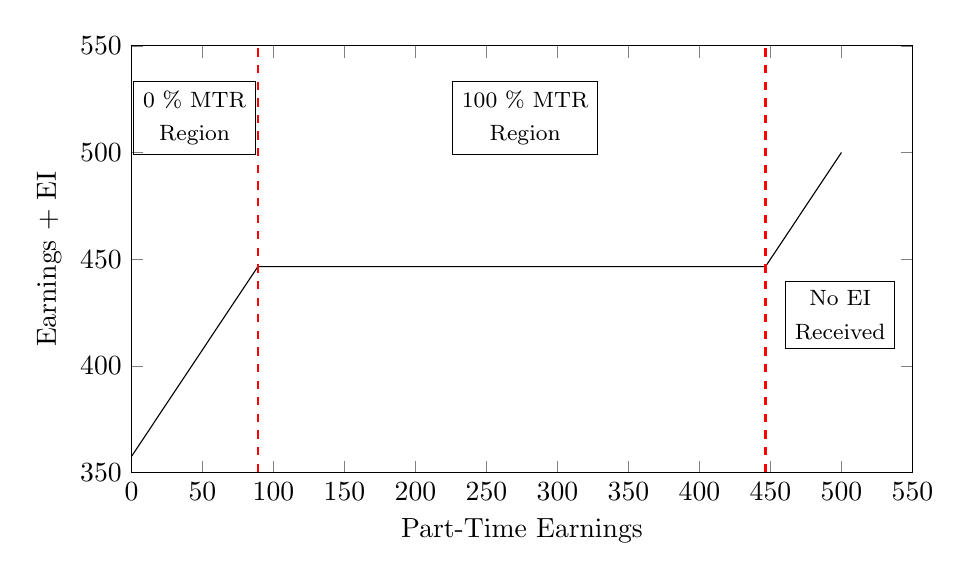
\begin{tikzpicture}
			\begin{axis}[xlabel = Part-Time Earnings, ylabel = Earnings + EI, height = 7cm, width = 11.5cm, xmin=0, xmax = 550, ymin=350, ymax = 550]
			\addplot[domain=0:550] coordinates { 
				(0,357.5)
				(89,446.5)
				(446.5, 446.5)
				(500,500)
			};
		
			\draw[red, thick, dashed] (89,0) -- (89,600);
			\draw[red, thick, dashed] (446.5,0) -- (446.5,600);  
			\end{axis}
			\node[draw, align=center] at (.8, 4.5) {\footnotesize 0 \% MTR \\ \footnotesize Region};
			\node[draw, align=center] at (5, 4.5) {\footnotesize100 \% MTR \\ \footnotesize Region};
			\node[draw, align=center] at (9, 2) {\footnotesize No EI \\ \footnotesize Received};
		\end{tikzpicture}
\end{frame}

\begin{frame}{Move from Threshold System to 50 \% Claw-Back on First Dollar Earned}
	\centering	\includegraphics[width=.9\linewidth]{../../figures/treatment2012_earningsw.pdf}	
\end{frame}

\section{Stepping Stone or Crowd-Out?}

\begin{frame}{How to Measure Causal Effect of Stepping-Stone}


\textcolor{blue}{IV Strategy?} Diff-in-Diff as IV for Part-time Work Propensity?


\begin{align*}
\underbrace{W_{i,q,r}}_{\textcolor{blue}{Work \ Propensity}} &=  \Pi \times \textcolor{blue}{D_{i,r}\times Post_{i,q,r}} + \eta_q + \eta_r  +  \varepsilon_{i,q,r} \\
\\
\underbrace{C_{i,q,r}}_{\textcolor{blue}{Claim \ Duration}} &= \textcolor{blue}{W_{i,q,r}} \bb{1}_{q=s} + \eta_q + \eta_r  +  \varepsilon_{i,q,r}
\end{align*}

\bigskip

\textcolor{blue}{Problem:} Treatment affects always-takers via liquidity. Screws up LATE.

\bigskip

\textcolor{blue}{What is policy relevant?} Reduced form elasticity?

\end{frame}


\section{Thanks!}


\appendix

\begin{frame}{Non-Parallel Trends in Claim Duration}
\begin{figure}
	\includegraphics[width=.8\linewidth]{../../figures/sample_selection100_swestern.png}
\end{figure}	
\end{frame}

\begin{frame}
	\begin{figure} \centering
		\begin{subfigure}{.42\textwidth}\centering\caption{\footnotesize Prob. Work With Benefits}\label{map1}
			\includegraphics[width=\linewidth]{../../figures/claim_spellparticipate_withbenefit.pdf}	
		\end{subfigure}
		\begin{subfigure}{.42\textwidth}\centering\caption{\footnotesize Prob. Work Without Benefits}\label{map2}
			\includegraphics[width=\linewidth]{../../figures/claim_spellparticipate_nobenefit.pdf}	
		\end{subfigure}
		\begin{subfigure}{.42\textwidth}\centering\caption{\footnotesize Avg Earnings With Benefits}\label{map1}
			\includegraphics[width=\linewidth]{../../figures/claim_spellearn_amt_withbenefit.pdf}	
		\end{subfigure}
		\begin{subfigure}{.42\textwidth}\centering\caption{\footnotesize Avg Earnings W-out Benefits }\label{map2}
			\includegraphics[width=\linewidth]{../../figures/claim_spellearn_amt_nobenefit.pdf}	
		\end{subfigure}
	\end{figure}
\end{frame}


\begin{frame}
	\begin{figure}
		\begin{subfigure}{.42\textwidth}\centering\caption{ \footnotesize Prob. Work With Benefits}\label{map1}
		\includegraphics[width=\linewidth]{../../figures/weeks_until_exitparticipate_withbenefit.pdf}
		\end{subfigure}
		\begin{subfigure}{.42\textwidth}\centering\caption{ \footnotesize Prob. Work W-out Benefits}\label{map2}
			\includegraphics[width=\linewidth]{../../figures/weeks_until_exitparticipate_nobenefit.pdf}	
		\end{subfigure}
		\begin{subfigure}{.42\textwidth}\centering\caption{ \footnotesize Avg Earnings With Benefits}\label{map1}
			\includegraphics[width=\linewidth]{../../figures/weeks_until_exitearn_amt_withbenefit.pdf}	
		\end{subfigure}
		\begin{subfigure}{.42\textwidth}\centering\caption{\footnotesize Avg Earnings W-out Benefits }\label{map2}
			\includegraphics[width=\linewidth]{../../figures/weeks_until_exitearn_amt_nobenefit.pdf}	
		\end{subfigure}
	\end{figure}
\end{frame}

\end{document}
